
%*****************************************
\chapter{Developing an Interaction System}\label{ch:forth}
%*****************************************
The following chapter represents an interaction system called \underline{\textbf{FiPa}} (\underline{\textbf{Fi}}nd \underline{\textbf{Pa}}ttern) which was developed to further examine the findings of Anonymous et al. \cite{anonymous}, discussed in Chapter \ref{ch:third}. Before entering into the development process, it is crucial to note that the following interaction system was created solely to serve as a tool in our user case study, which will be presented in Chapter \ref{ch:fifth}. The system is in no means a suggestion for an authentication concept and was not intended to be utilized as such. Its sole purpose was meant for the scope of this thesis, and no further. Therefore certain aspects (e.g., security and effectiveness) have consciously not been considered during the design and the development of this system. Nonetheless, the design process was based on a  \textbf{User-Centered Design} (UCD) approach and included a selection of \textbf{Human Computer Interaction} (HCI) principles, to make the system easier to understand and function. The exact procedure of this process will be documented through the direct voice of the author to convey her thought process and intentions in this part of her contribution towards this thesis. 

\section{Requirements of the Concept} \label{4.1}
As mentioned above, the interaction system was intended to be utilized as a tool to help examine certain factors later on in our study. These factors are \textit{orientation time} and \textit{input time}, previously introduced in Chapter \ref{ch:third}. In order to do so, our interaction system had to be based on a certain concept. This concept had to be divided into two coherent and related small tasks: a \textbf{mental task} and a \textbf{practical task}. The intention behind this division was to be able to measure the \textit{orientation time} (duration of the mental task) and the \textit{input time} (duration of the practical task), separately. For that, a timer feature had to be implemented, in order to undertake the measurements, which would automatically be saved in a local database (see Section \ref{4.3}).\\


Based on the findings by Anonymous et al. \cite{anonymous} (see Chapter \ref{ch:third}), I was interested in examining the impact that the \textit{orientation time} had on the perceived efficiency of an authentication concept, with respect to its \textit{input time}. We, therefore, decided to analyze the following two contrasting time ratios:  
\begin{center}
    "\textcolor{blue}{long} orientation/\textcolor{red}{short} input" \\
    \textbf{vs.} \\
    "\textcolor{red}{short} orientation/\textcolor{blue}{long} input".
\end{center} 

The crossing descriptors \textit{long} and \textit{short} were set to define a certain length, meaning \textit{long orientation} had to have the same duration as \textit{long input}, and vice versa. 

In order to have a baseline to which the measured times of the ratios above could be compared, I included a third ratio, where \textit{orientation time} and \textit{input time} were equally long. We will call this ratio \textcolor{red}{short} orientation/\textcolor{red}{short} input. \\
 

In addition to the study by Anonymous et al. \cite{anonymous}, I was interested in directly comparing both contrasting ratios against each other by using \textit{only one concept}, instead of three (see Chapter \ref{ch:third}). Through unifying all three ratios into one concept, it was possible to eliminate the chance of future results being influenced by the study participants' personal preferences of the concepts.
For that reason, the created concept had to be malleable in a way, such that the complexity of each tasks (\textbf{mental} and \textbf{practical}) could be adjusted, according to the represented ratio. This meant, the less difficult and the less complex a task was, the lesser time it needed to be accomplished, and vice versa. 

\begin{figure}[t!]
\centering
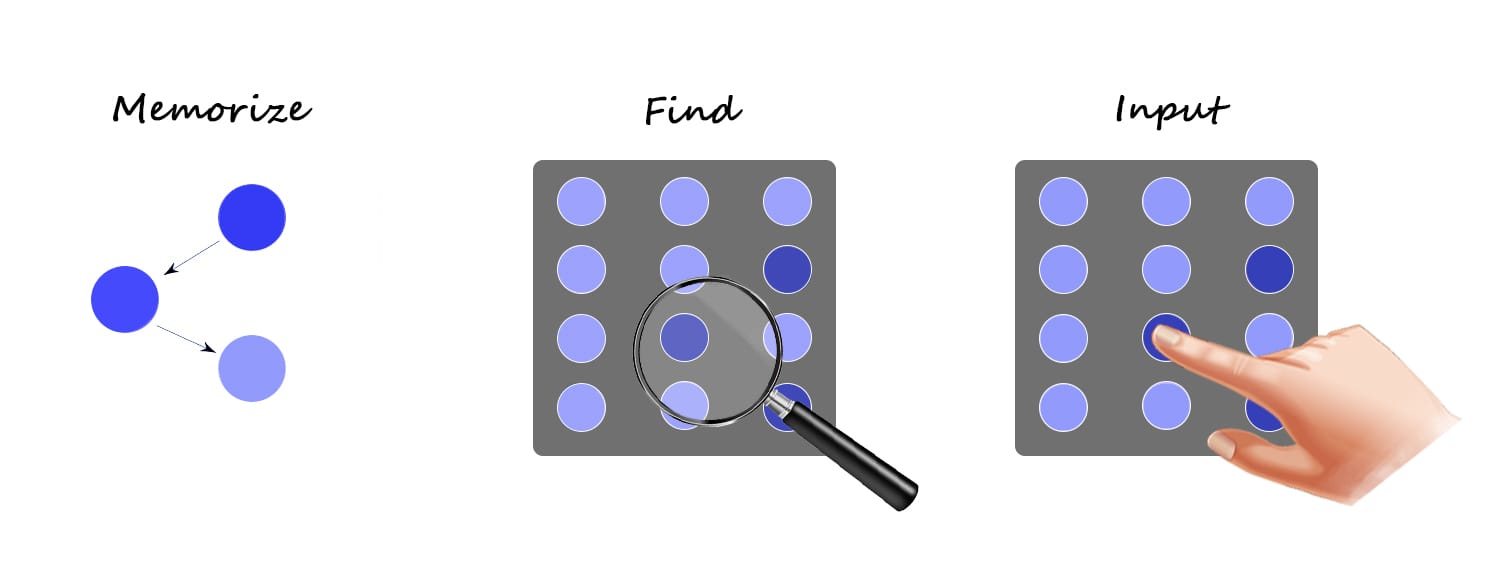
\includegraphics[width=15cm, height=6cm]{Chapters/graphics/ConceptIdea.jpeg}
\caption{Simple illustration of the idea. The procedure is composed of three steps: \textbf{Memorize} a pattern, \textbf{Find} the pattern, hidden inside a grid, and then \textbf{Input} of the pattern.}
\label{fig:concept}
\end{figure}

\section{Concept Development} \label{4.2}

In the following section, we will present the design and evaluation attempts that were necessary to generate \underline{\textbf{FiPa}}: the interaction system presented and utilized in our study. 

\subsection{Fundamental Concept Idea} \label{4.2.1}

I were interested in creating a concept which activated an interaction that believably resembled a smartphone authentication. I assumed that by making the interaction resemble an authentication process, future study participants could better understand and adapt to the context of the study. One of our goals was to construct a concept that was as usable as possible. That way, we could shine light on the actual usability issues which we intended to examine. We, therefore, decided to create a \textit{graphic-based concept}, as they are perceived as most user-accepted and most comfortable to use, on average \cite{PatternWild}. \\ 

The name of our concept, \underline{\textbf{FiPa}}, is inspired by its functionality. \underline{\textbf{FiPa}} is an abbreviation for the phrase "\underline{\textbf{Fi}}nd \underline{\textbf{Pa}}ttern" and its meaning will be comprehensible through the following description of its procedure (see figure \ref{fig:concept}): First, a predefined pattern is presented which has to be memorized well by the user. This pattern consists of a certain combination of buttons. Each button has a certain characteristic, that makes it distinguishable from the others. Memorizing the order of the buttons and their distinct characteristics is crucial for successfully accomplishing the \textbf{mental} and \textbf{practical task} (Section \ref{4.2.1}). After \underline{memorizing} the pattern, a large grid, filled with buttons, is presented. The \textbf{mental task} thereby is to \underline{find} the memorized pattern, hidden inside the grid. When found, the \textbf{practical task} is comprised of entering  (\underline{input}) the found pattern correctly into the grid (see figure \ref{fig:concept}).\\


We derived the idea of using a grid of buttons from the concept \textit{Pattern Rotation} \cite{Marbles, anonymous}. The choice of using specific characteristics for each button was inspired by the concept \textit{Marbles} \cite{Marbles, anonymous}. We tried to limit the amount of mental effort required for interacting with our concept by making a few intentional design choices. We imagined that having to reproduce the memorized pattern for the input, would be tiresome and not possible for every participant, especially if the pattern was long. We also took into consideration that the pattern would most certainly not be memorized permanently and would, therefore, be stored in participants' short-term memory. To that, we assumed that having to search for the pattern would require less mental effort than its complete reproduction. That way, during the mental task, when the user stumbles upon the hidden pattern in the grid, they are more likely to detect it because they recognize it. So, by decreasing the amount of mental effort required for the interaction with the concept, we hoped that our participants would be able to shift their focus onto the ratios represented in the study.

\begin{figure}[t!]
\centering
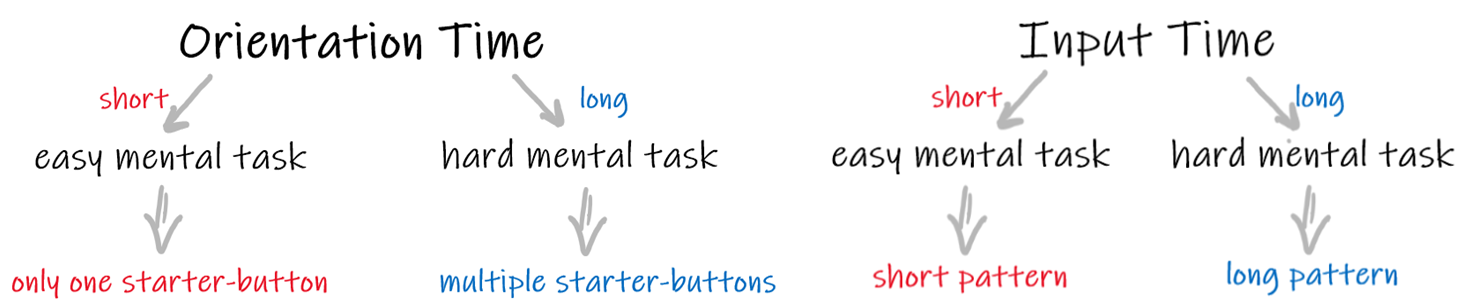
\includegraphics[width=13cm, height=4cm]{Chapters/graphics/OriInput.PNG}
\caption{Depiction of how we attempted to construct the mental and practical tasks, depending on whether \textbf{orientation time} and \textbf{input time} were long or short.}
\label{fig:orientation_input}
\end{figure}


\subsection{Concept Design} \label{4.2.2}
In the following we will present the design approaches that lead us to creating and developing the interaction system \underline{\textbf{FiPa}}.

\subsubsection{First Draft} \label{4.2.2.1}
We illustrated our initial vision for the design in figure \ref{fig:firstdraft}. As in \textit{Marbles} \cite{Marbles, anonymous}, we decided to make the different elements of our concept (the buttons) distinguishable through small images, emojis to be exact. We will first begin by explaining how we visualized the \textbf{practical task} and then proceed with explaining our intentions regarding the \textbf{mental task}. As mentioned in Section \ref{4.1}, a pattern is required to be memorized at the very beginning of the activity. To mark the beginning of a pattern, we determined the first button of each pattern to contain a key-emoji (see figure \ref{fig:firstdraft}). We will call this button the \textit{starter-button}. In order to modify whether the intended \textbf{input time} should be short or long, we created examples of how we imagined the patterns should look like in Figure (see figure \ref{fig:firstdraft}). Similar to the input method in \textit{Android Unlock Pattern}, we decided the user would enter the pattern by connecting the buttons with their finger. We found this input method to be more suitable, being that \underline{\textbf{FiPa}} was intended to be a smartphone application and that the user would interact with it through a touch screen. \\

As for the \textbf{mental task}, we envisioned to design a grid filled with emoji-buttons. The design of the grid depended on whether long \textit{orientation time} or short \textit{orientation time} was intended. As mentioned earlier in Section \ref{4.1}, we assumed that for a long \textit{orientation time}, we need to create a difficult and more complex search process. We imagined that by incorporating multiple \textit{starter-buttons} inside the grid, besides the one belonging to the hidden pattern, we could complicate and elongate the search process. In contrast, we imagined it would be possible to facilitate the pattern search, by having the only \textit{starter-button} in the grid belong to the hidden pattern. That way, our future participants could spot the pattern much easier and quicker. 

\begin{figure}[t!]
\centering
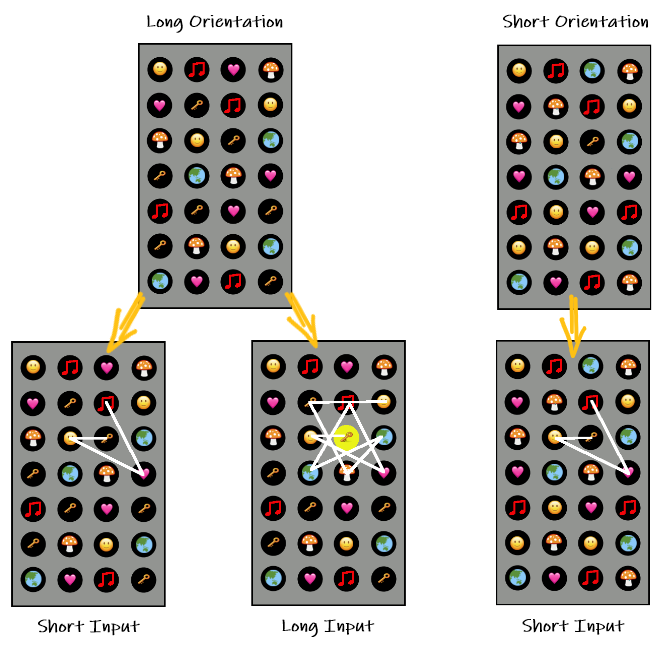
\includegraphics[width=14cm, height=14cm]{Chapters/graphics/firstdraft.PNG}
\caption{More detailed representation our vision for the design and the construction of the mental and practical tasks in our concept.    }
\label{fig:firstdraft}
\end{figure}

\subsubsection{Evaluation: First Draft} \label{4.2.2.2}
In order to find out if our concept was effective in practice, we created a paper prototype. The prototype encompassed the three ratios (Section \ref{4.1}) and was composed of three patterns\footnote{Two short patterns intended for \textit{short input time} and one long pattern intended for \textit{long input time}.} and three grids\footnote{Two grids with only one \textit{starter-button}, for \textit{short orientation time} and one grid with multiple \textit{starter-buttons}, for \textit{long orientation time}.}. We used the same grid and pattern design shown in figure \ref{fig:firstdraft}. \\
It was important for us to see how our design affected the usability of our concept. We wanted to ensure that it was easy to use and easy to understand. So, we recruited six participants to evaluate our concept. Before the interaction, we roughly explained the purpose of our study and the functionality of our prototype. We used a form of \textit{Wizard Of Oz} prototyping \cite{Butz2014}. During the interaction, we would uncover the following event of the prototype (grid or pattern), depending on the participant's \textit{input} or \textit{action}. We timed the interaction for each user in a specific manner, using a stopwatch. Our intention was to ensure that the accomplishment of the \textbf{mental task}, designed for long \text{orientation time}, truly took longer than the ones intended for short \textit{orientation time}. The same was important for the \textbf{practical tasks} and their corresponding \textit{input times}. We wanted to measure the ratios similar to the approach made by Anonymous et al. \cite{anonymous} (see Chapter \ref{ch:third}). So, we defined a distinct intervall for each of the tasks. A \textbf{mental task} began right after a particular grid was uncovered and ended as soon as the hidden pattern was found. The find was indicated by tapping the \textit{starter-button} of the pattern once. The \textbf{practical task} began with the \textit{first button press} and ended with the very \textit{last button press}.  For the input, the \textit{starter-button} had to be incorporated, although it had previously been tapped to signify the find. We were aware that the measured times would not be completely accurate. They were only intended to serve as a rough estimates for the duration of the phases.\\


Five of the participants considered the emojis to be overwhelming on the eyes. They found that it made the grid appear very crowded. Moreover, the long pattern was considered too complicated and was hard to memorize by all of the participants (see figure \ref{fig:firstdraft}). Regarding the input method, we noticed that it was not suitable for the realization of the different \textit{input time} variations. Although it worked well for short \textit{input time}, the time needed to enter the long pattern was not as long as we had intended for it to be.
Luckily, the idea behind the concept was liked by all of the participants. Especially, the notion of starting each pattern with a specific \textit{starter-button}. Despite the flaws mentioned above, they understood the basic functioning of our concept well. \\

The information gained and the lessons learned through the previous evaluation phase gave us a closer insight into humans' perception and cognitive ability. At this point, we were one step closer to creating a more usable and effective interaction system.

\begin{figure}[t!]
\centering
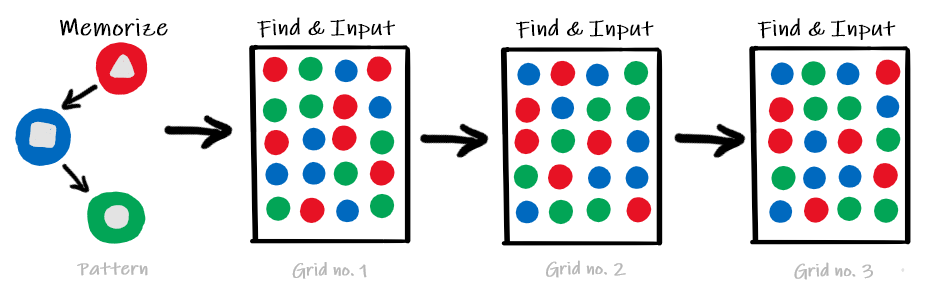
\includegraphics[width=13cm, height=5cm]{Chapters/graphics/seconddraft.PNG}
\caption{A sketch that presents the basic structure of each phase of the prototype. Each grid represents a \textbf{couple}: a mental and a practical task. After memorizing the given pattern, three uniquely designed grids followed. The pattern had to be found and entered in each of the grids, one after the other.}
\label{fig:secondDraft}
\end{figure}

\subsubsection{Second Draft} \label{4.2.2.3}

We decided to make a few adjustments regarding the overall aesthetics and the design of our concept. Through further research, we learned that due to the \textit{pictorial superiority effect} \cite{pictorial}, humans can retain information through images, much better than through letters or numbers \cite{pictorial, 2014}. That is why we chose to continue representing the characteristics of the buttons through images. We decided to reduce the crowded appeal of the previous draft by replacing the emojis with three simple shapes: \textit{circle}, \textit{square}, and \textit{triangle}. Our initial choice of colors for the design was: \textit{red}, \textit{green} and \textit{blue}. The reason for our choice is that they are the basic colors that the human eye perceives naturally \cite{Butz2014}. We kept the notion of each pattern, beginning with a \textit{starter-button} and decided for it to be a red button containing a triangle, as illustrated in [FIGURE]. We chose the triangle because it is a symbol that has been shown to convey the meaning of \textit{power}\footnote{http://www.whiteriverdesign.com/meaning-shapes-design/ - last accessed: 2019/11/16} and \textit{permanence} \cite{Frutiger1998}.  Moreover, the human eye is naturally attracted to its shape \footnote{https://designshack.net/articles/layouts/the-sometimes-hidden-meaning-of-shapes/ - last accessed: 2019/11/16}. We assumed that through the mentioned effect of the triangle and the alerting appeal of the color red, we could attract the user's \textit{pre-attentive perception} \cite{Butz2014} to these buttons. \\

Next, we proceeded with designing the pattern and grid design. After a couple of trials, we determined the size of the grid to be 4x7, because we found that the size was suitable to hold a decent amount of buttons and yet sufficiently big for participants to have a clear overview of the grids content. Also, we decided to incorporate so-called \textit{traps} into the grids. \textit{Traps} are a set of buttons, that have a similar constellation and set of characteristics as the hidden pattern, yet are not identical to it. Their purpose is to mislead the user, during the \textbf{mental task} and thereby elongate the search process when needed. Another modification made was the input method. We found that by tapping all of the buttons in the right order, instead of connecting them (see Section \ref{4.2.2.1}), we could gain more control of the approximate duration for the input even better. During the creation of the patterns, it was crucial that they did not cover too much space inside grid, such that we could shuffle the buttons and set \textit{traps} more freely. 

\begin{figure}[t!]
\centering
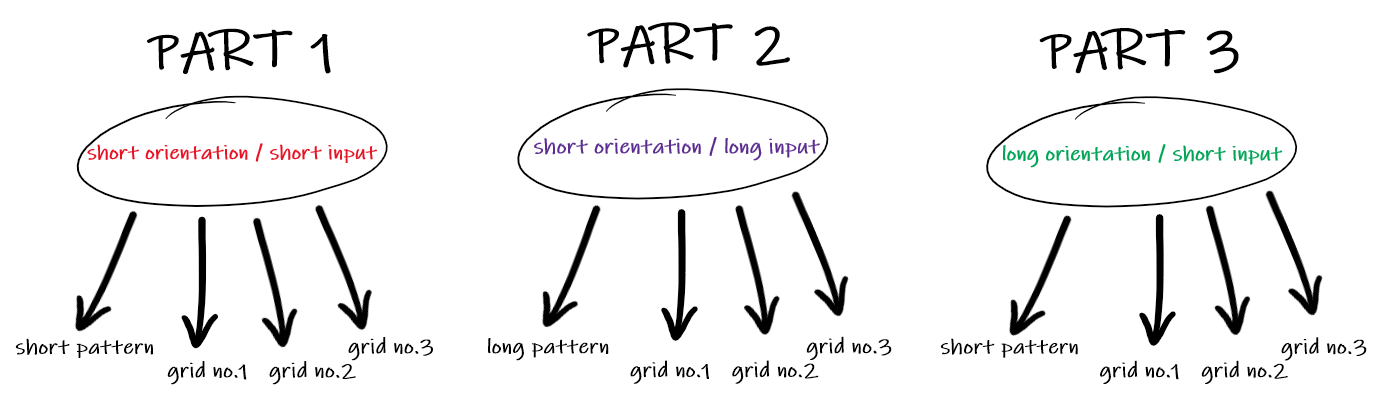
\includegraphics[width=13cm, height=5cm]{Chapters/graphics/prototypeStructure.PNG}
\caption{Simple representation of the structure of our second design. Each part is assigned to a particular ratio. For each ratio there are three grids. Each grid presents a \textbf{mental task} (find) and \textbf{practical task} (input), a so called \textbf{couple}. The order of the ratios presented in this figure is only a suggestion. The exact order of the ratios was not important in the evaluation phase.}
\label{fig:prototype}
\end{figure}

\subsubsection{Evaluation: Second Draft} \label{4.2.2.4}

As in our first draft evaluation (see Section \ref{4.2.2.2}), we created a \textit{Wizard of Oz} paper prototype \cite{Butz2014} to evaluate the changes and improvements that we made in our concept. However, this time, the prototype was created differently. We wanted to test a certain structure to see if it would be suitable for the implementation of our concept as an interaction system. The prototype was structured into \underline{three parts} thus, we had three ratios (see Section \ref{4.1}) to examine. In the previous draft, we only had one \textbf{mental} and \textbf{practical task} per ratio. For simplicity, we will call the composition of \textbf{mental} and \textbf{practical task}, a \textbf{couple}. Instead of having only one \textbf{couple} per ratio (as in the first draft), we decided it would be reasonable to assign three to each ratio. We assumed our participants would have the chance to interact with each ratio-designs more than once and remember them better during the qualitative segment of our study. Figure \ref{fig:prototype} represents the rough structure of our paper prototype. We tested our prototype with the same set of participants with whom we had tested our first draft. We did so, in order to receive a more detailed feedback on whether the flaws, detected in our first draft, were correctly fixed. It was possible to interview the same set of participants because the design and the structure of the \textbf{mental} and \textbf{practical tasks} were completely different than in the first draft. Fortunately, both, layout and structure of our prototype were well accepted. \\

We adapted the same measurement method that we used in Section \ref{4.2.2.2}. We considered the first and second couple of each part to be an exercise for the participant to get acquainted with the concept. So, we only considered the average times of each third couple of each ratio. Although not accurate, the approximate duration resulted as we had imagined and desired for our concept.

\section{Implementation of the Concept} \label{4.3}

The following section will present the implementation of our concept and the creation of the interaction system \underline{\textbf{FiPa}}. We will explain the structure of the application and certain features which we embedded into it. \underline{\textbf{FiPa}} was solely intended to be a supportive tool to help us validate the findings made by Anonymous et al. \cite{anonymous}, later in our complementary study (see Chapter \ref{ch:fifth}). For that, we will not deal with exact details of its framework, to avoid distraction from the fundamental purpose of our thesis.\\

\underline{\textbf{FiPa}} was implemented as an Android application, using the Software \textit{Android Studio}, which is based on IntelliJ IDEA. It is comprised of a series of classes, called activities. They can be seen as the fundamental building blocks of an application. Each activity describes and controls the functions of the user interface (UI) presented in that window\footnote{https://developer.android.com/guide/components/activities/intro-activities - last accessed: 2020/01/03.}. The structure of the UI is defined by a so-called layout, which is an XML-file that defines the features (i.e., images, buttons, strings) presented in a particular window\footnote{https://developer.android.com/guide/topics/ui/declaring-layout - last accessed: 2020/01/03.}. Activities within an application are able to communicate with each other and they determine the following event of each action in a window. 

\subsection{Structure} \label{4.3.1}

Analoguous to the prototype of our second draft (see Section \ref{4.2.2.4}), our application consisted of \underline{three parts}. In the application they were called phases, which is not to be confused with Anonymous et al.'s \cite{anonymous} notion for the term phase, in Chapter \ref{ch:third}. 

The elemental structure of the application was first assessed by creating a simple illustration using cards [FIGURE]. The itention behind this approach was to We did this to create a precise conception of activity flow would be and to think of a strategy to accurately measure the times of \textit{orientation} and \textit{input}. Analogous to the design of our prototype, presented in Section \ref{4.2.2.4}, we intended that the application consisted of \underline{three distinct parts}. Each part represented a distinct ratio, called a \textit{phase}\footnote{Not to confuse with Anonymous et al.'s interpretation of a phase, in Chapter \ref{ch:third}.}. 
In our previous prototype, each \underline{part} consisted of three \textbf{couples} (a combination of \textbf{mental} and \textbf{practical task}). Therefore we divided each of the \textit{phases} into three \textit{levels}, each representing a \textit{couple}. Moreover, each \textit{phase} has a pattern (either short or long) assigned to it. \\

All phases have the same flow. The first activity of each phase shows an assigned pattern on the screen. The order in which the buttons should be entered is conveyed through a simple animation. When the pattern is memorized, the user can proceed by pressing a green \textit{"READY"}-button. The next activity presents a layout with a green squared \textit{"START"}-button. This activity is of great importance as it defines the starting point of the \textbf{mental task}, meaning the beginning of the \textit{orientation phase}. The measurement of the \textit{orientation time} is initiated as soon as the \textit{"START"}-button is pressed and ends in the next activity, as soon as the user taps the correct \textit{starter-button}. This action causes a transformation: All buttons in the grid are blended out, except for the ones belonging to the pattern. The transformation is meant to convey to the user that they can execute the \textbf{practical task}, meaning the \textit{input phase}. The measurement of the \textit{input time} is initiated through the first button-press, given that the correct \textit{starter-button} is selected, and ends when the last button of the pattern is pressed, given the pattern was entered correctly. If not, the time for \textit{input phase} cannot be stored in the database, and is marked as \textit{"failed"}. Analogous to the prototype, in Section \ref{4.2.2.4}, the \textit{starter-button} was meant to be pressed twice: Once to signify the find of the pattern and end the measurement of \textit{orientation time}, and once again to initiate the beginning of the \textit{input phase}. 

This process\footnote{Here we distinctively mean the process starting with the \textit{START}-button onward.} repeats itself for the following two levels of each phase. At the end of each phase the following phase automatically begins by presenting the next pattern [FIGURE].

\subsection{Application Flow and Features} \label{4.3.2}

In the following section, we will present the flow of our application \underline{\textbf{FiPa}}, whilst introducing its special features along the way. \\

The first activity of the application presents window which allows the user to choose whether they would like to proceed with the training-segment or skip to the study. Assume we were to proceed with the training. The training segment presents an exercise walk-through of the concept, meant to get the user acquainted with the concept of \underline{\textbf{FiPa}} and to minimize the amount of errors made throughout the study. At the end of the training-segment, users have the option to proceed with the study or repeat the training. We wanted to assure that users truly understood the functioning of the concept which is why they had the freedom to repeat the training-segment as often as they felt necessary. Assume we were to proceed with the study. The next activity is responsible for the maintenance of the collected data. It allows to enter a user-id for the user, which helped to pair a user's collected quantitative data (measurements) with their qualitative data (survey answers) later in evaluation. Moreover, it was possible to view the content of the local database through the application. This feature was useful during the development of the application, to assure that the phases were measured correctly, and also in many cases during the study. From this point, let us assume we were to start the study. This action would lead us to the first phase of the concept. As described in Section \ref{4.3.2}, each phase begins by presenting its corresponding pattern, intended for memorization. When the pattern is memorized, the user can proceed by pressing the \textit{"READY"}-button. It is important to note that buttons, used to approve or proceed, were intentionally given the color green, as it is it is commonly associated with the action "GO" or the approval "OK" in everyday life. \\

Assume we were to proceed and begin with the Level 1 of Phase 1. At this point, we have to complete the \textbf{mental task}, which is to find the hidden pattern inside the grid. During the search process, the \textit{orientation time} is being measured in the background. The measurement is unnoticeable to the user during the interaction. As it is possible to press the wrong starter-button during the search process, we added a feature into the application which served as a form of \textit{error-recovery} (see Chapter \ref{ch:third}). It was realized through a pop-up window which appeared after the third search error was made. The pop-up illustrated the pattern to remind the user, in case they had forgotten it. As soon as the user found the pattern, the grid transformed as described in Section \ref{4.3.1}, signifying the beginning of the \textbf{practical task}. As errors were also possible during the input, we also included \textit{error-recovery}. Here, the pop-up window appeared after the third input error. After it appeared, the app proceeded with the next action and marked the input of the particular level as \textit{"failed"}. Although the main focus is to examine the effects of \textit{orientation time} and \textit{input time}, we could not avoid including an \textbf{error-recovery phase}, as it would have negatively impacted the user-friendliness of the application\footnote{To assure that the \textit{error-recovery phase} did not have an impact on the results of our study, we took specific measures, which will be presented in Chapter \ref{ch:fifth}.}. The procedure of the two follow-up levels of the phase have the same presented procedure. The flow of the two following phases is analogous to the presented one. ADD FLOW CHART HERE SOMEWHERE !!  \\

As it is crucial for the study that the phases of the application, which represent the different time ratios, are counterbalanced amongst the participants, we decided to permute them manually by changing the order of the activities in the code of the study-segment. As previously mentioned, the implemented local database of the application measured the beginning and the end of both, \textit{orientation} and \textit{input phase}\\

The next chapter will 



